\documentclass{beamer}
\mode<presentation>
{
  \usetheme{Madrid}     
  \usecolortheme{crane} 
  \usefonttheme{default}  
  \setbeamertemplate{navigation symbols}{}
  \setbeamertemplate{caption}[numbered]
} 

\usepackage[english]{babel}
%\usepackage[utf8x]{inputenc}
\usepackage{CJKutf8}
\usepackage{graphicx}
\usepackage{amsmath}

\title[M-NMT]{Memory-augmented Neural Machine Translation}
\subtitle{Paper Review}
\author{Bojan Bo\v{z}i\'{c}}

\begin{document}

\begin{frame}
  \titlepage
\end{frame}

\section{Introduction}
\begin{frame}{Introduction}
\begin{itemize}
  \item NMT has highly promising performance for large training data.
  \item Common principle: encoding meaning of input into concept space and performing translation based on encoding $\rightarrow$ deeper understanding and learning of translation rules, better translation than SMT. 
  \item Problem: tendency towards overfitting to frequent observations and overlooking special cases.
  \item Cause: Translational function is shared, so high- and low-frequency pairs impact each other by adapting shared parameters. Smoothness of translation function makes infrequent pairs seem like noise.
\end{itemize}
\vskip 0.1cm
\begin{block}{Neural Machine Translation}
Is an approach to machine translation that uses a large neural network. It departs from phrase-based statistical approaches that use separately engineered subcomponents. E.g. Google uses Google Neural Machine Translation (GNMT) in preference to its previous statistical methods.
\end{block}
\end{frame}

\begin{frame}{Problem: Low-frequency pairs}
\begin{table}
\begin{tabular}{ll}
\hline
\textit{src.} & \begin{CJK}{UTF8}{gbsn}人类共有二十三对染色体。\end{CJK}\\
\textit{ref.} & Humans have 23 pairs of chromosomes.\\
\textit{NMT} & There are 23-year history of human history.\\
\hline
\end{tabular}
\caption{An example of Chinese-to-English meaning drift with NMT.}
\end{table}
\end{frame}

\begin{frame}{Errors}
\centering
\begin{tabular}{cc}

\includegraphics[width=5cm]{error1} & 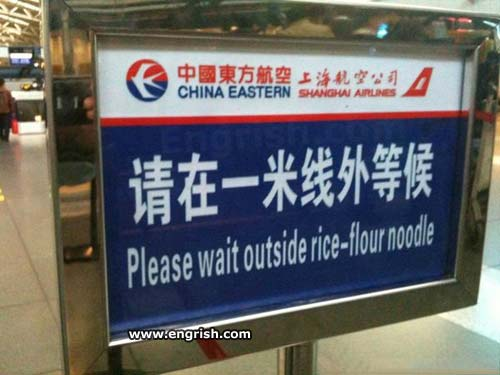
\includegraphics[width=5cm]{error2}\\
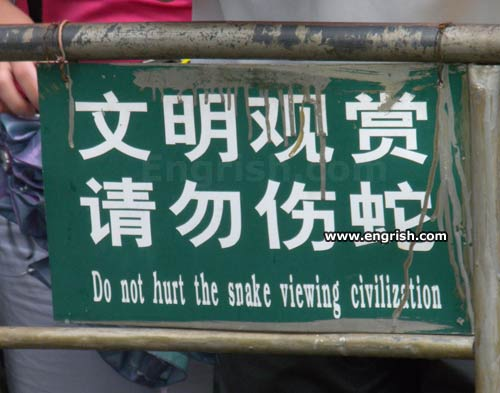
\includegraphics[width=5cm]{error3} & 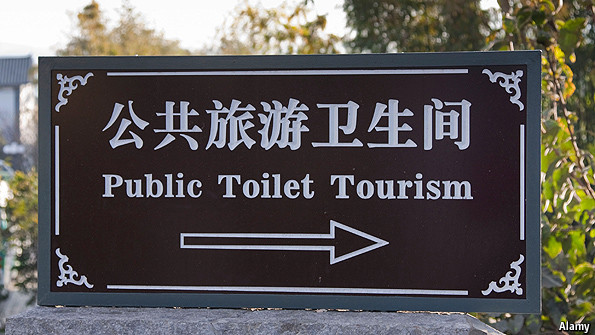
\includegraphics[width=5cm]{error4}
\end{tabular}
\end{frame}

\begin{frame}{Statistic Machine Translation}
\begin{itemize}
\item Based on statistics of words and phrases (i.e. symbolic method with discrete model).
\item Discrete model = probability of infrequent pairs cannot be smoothed out.
\item Lack of shared parameters = frequent pairs have much less impact on infrequent pairs.
\item SMT memorises as many observed patterns as possible by using a phrase table.
\item Ideal: Neural model with complementary statistical support.
\end{itemize}
\end{frame}

\section{Attention-based NMT}
\begin{frame}{Attention-based NMT}
\begin{itemize}
\item Attention-based RNN model with encoder-decoder frame is used.
\item MLP similarity function: $\alpha_{ij}=\frac{e_{ij}}{\sum{e_{ik}}}; e_{ij}=a(s_{i-1},h_j)$
\item Semantic content: $c_i=\sum{\alpha_{ij}h_j}$
\item Update with recurrent function: $s_i=f_d(y_{i-1},s_{i-1},c_i)$
\item Next word: $p(y_i)=\sigma(y_i^TWz_i)$
\item Intermediate variable: $z_i=g(y_{i-1},s_{i-1},c_i)$
\end{itemize}
\end{frame}

\subsection{Memory-augmented NMT}
\begin{frame}{M-NMT Architecture}
\begin{figure}
\centering
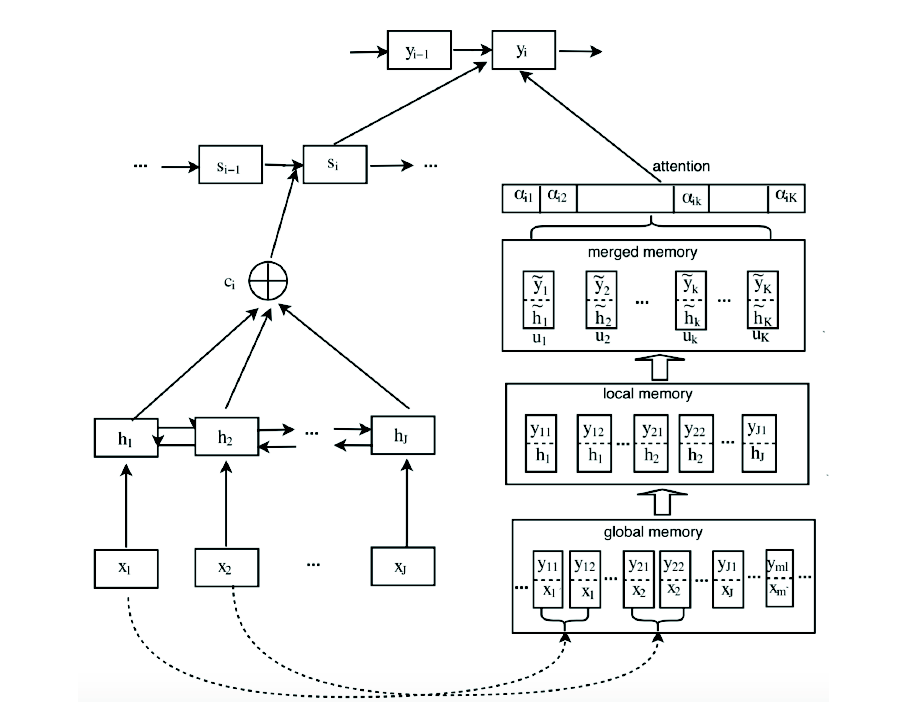
\includegraphics[width=9cm]{m-nmt-arch}
\caption{The structure of the M-NMT architecture.}
\end{figure}
\end{frame}

\begin{frame}{Memory Elements}
\begin{itemize}
\item Attention-based RNN model is good with frequent words, and memory elements provide knowledge of infrequent words.
\item Memory element: $u_{jl}=\begin{bmatrix}y_{jl}\\x_j\end{bmatrix}$
\item Local memory: $u_{jl}=\begin{bmatrix}y_{jl}\\h_j\end{bmatrix}$
\item Compression: $u_k=\begin{bmatrix}\tilde{y}_k\\\tilde{h}_k\end{bmatrix}=\begin{bmatrix}\tilde{y}_k\\\sum_j{p(x_j|\tilde{y}_k)h_j}\end{bmatrix}; \forall\tilde{y}_k\in\{y_{jl}\}$
\end{itemize}
\end{frame}

\begin{frame}{Memory Attention}
\begin{itemize}
\item Attention factor: $\alpha^m_{ik}=\frac{e^m_{ik}}{\sum^K_{k=1}{e^m_{ik}}}$
\item Relevance function: $e^m_{ik}=(v^m)^Ttanh(W^m_ss_{i-1}+W^m_uu_k+W^m_yy_{i-1})$
\item Consolidated posterior: $\tilde{p}(y_i)=\beta\alpha^m_{ik}+(1-\beta)p(y_i)$
\item Objective function: $$L(\theta)=\sum_n{\sum_i{log(\alpha^m_{ik^n_i})}}$$
\end{itemize}
\end{frame}

\begin{frame}{Memory Integration}
\begin{itemize}
\item Translation dictionary produced by SMT system is used.
\item Align training sentence pairs using GIZA++ and apply intersection refinement rules to get a single 1:1 alignment for each sentence pair and extract translation dictionary.
\item Key information is conditional probability that source and target word are translated to each other. This is used twice:
\begin{enumerate}
\item conditional $p(y_{jl}|x_j)$ used to select target words $y_{jl}$
\item conditional $p(x_j|\tilde{y}_k)$ used to merge element with target words $\tilde{y}_k$
\end{enumerate}
\end{itemize}
\end{frame}

\begin{frame}{OOV Treatment}
\begin{itemize}
\item Manually defined dictionary specifies how to translate OOV words.
\item Use this to construct local memory at run-time.
\item When OOV is encountered the vector of a similar word is borrowed.
\item Alternative choices should prevent collisions of the similar word.
\item Problem: Vocabulary of neural model is fixed  $\rightarrow$ no probabilities.
\item Solution: Rewrite similar word by OOV word and redirect prediction. 
\end{itemize}
\end{frame}

\subsection{Experiments}
\begin{frame}{Experiments}
\begin{itemize}
\item Two datasets: small IWSLT (44k sentences from tourism domain) and large NIST (1M sentence pairs from LDC corpora)
\item Memory construction: GIZA++ toolkit
\item Baselines: conventional SMT and attention-based RNN NMT
\end{itemize}
\end{frame}

\begin{frame}{M-NMT Configurations}
\begin{table}
\centering
\begin{tabular}{|l|l|l|}
\hline
System & Attending & Attended \\
\hline
$M-NMT(s,u^y)$ & $s_{i-1}$ & $u_k(y)$ \\
$M-NMT(s,u^{xy})$ & $s_{i-1}$ & $u_k(x),u_k(y)$ \\
$M-NMT(sy,u^y)$ & $s_{i-1},y_{i-1}$ & $u_k(y)$ \\
$M-NMT(sy,u^{xy})$ & $s_{i-1},y_{i-1}$ & $u_k(x),u_k(y)$ \\
\hline
\end{tabular}
\caption{M-NMT systems with different configurations.}
\end{table}
\end{frame}

\begin{frame}{BLEU Scores}
\begin{table}
\begin{tabular}{|l|c|c|}
\hline
System & IWSLT05 & NIST03 \\
\hline
Moses & 52.5 & 30.6 \\
\hline 
NMT & 43.9 & 31.3 \\
\hline
NMT-L & 45.9 & 31.7 \\
\hline
$M-NMT(s,u^y)$ & 49.8 & 32.3 \\
$M-NMT(s,u^{xy})$ & 50.7 & 32.5 \\
$M-NMT(sy,u^y)$ & 51.4 & 32.8 \\
$M-NMT(sy,u^{xy})$ & \textbf{52.9} & \textbf{34.0} \\
\hline
\end{tabular}
\caption{BLEU scores with different translation systems on the two Chinese-English translation datasets.}
\end{table}
\end{frame}

\begin{frame}{OOV Recall Rates}
\begin{table}
\begin{tabular}{|l|c|c|c|c|}
\hline
& \multicolumn{2}{|c|}{T-INV} & \multicolumn{2}{|c|}{T-OOV} \\
\hline
System & Recall & BLUE & Recall & BLEU \\
\hline
NMT & 0.06 & 15.1 & 0 & 13.7 \\
\hline
M-NMT & 0.05 & 16.0 & 0 & 14.6 \\
\hline
NMT-PL & 0.09 & 15.4 & 0.08 & 14.3 \\
\hline
M-NMT+OOV & \textbf{0.28} & \textbf{17.0} & \textbf{0.40} & \textbf{15.9} \\
\hline
\end{tabular}
\caption{The OOV recall rates and BLEU scores on sentences with OOV words. ‘T-INV’ refers to the case where the target words of the OOV input are in-vocabulary, and ‘T-OOV’ means the case where the target words are also OOV.}
\end{table}
\end{frame}

\begin{frame}{Word Frequency}
\begin{figure}
\centering
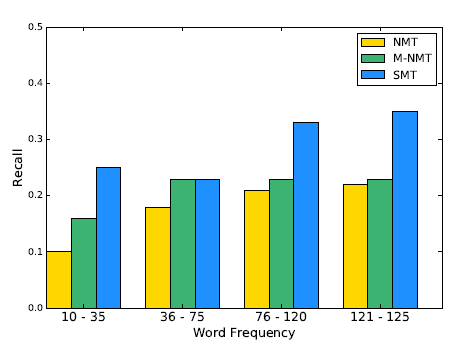
\includegraphics[width=9cm]{recall}
\caption{The recall rates of words in different frequency bins.}
\end{figure}
\end{frame}

\begin{frame}{Translation Results}
\begin{table}
\centering
\begin{tabular}{ll}
\hline
\textit{src.} & \begin{CJK}{UTF8}{gbsn}人类共有二十三对染色体。\end{CJK}\\
\textit{ref.} & Humans have 23 pairs of chromosomes.\\
\textit{Moses} & A total of 23 human chromosome.\\
\textit{NMT} & There are 23-year history of human history.\\
\textit{M-NMT} & There have a total of 23 species of chromosomes.\\
\hline
\end{tabular}
\caption{The translations from different systems for the Chinese-to-English ‘meaning drift’ example.}
\end{table}
\end{frame}

\subsection{Conclusion}
\begin{frame}{Conclusion}
\begin{figure}
\centering
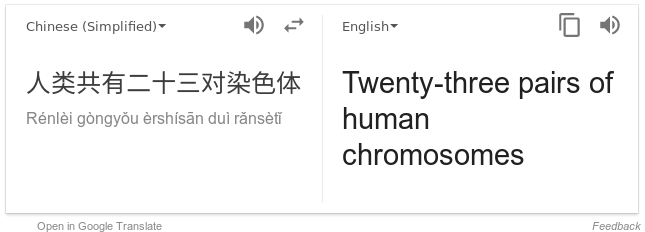
\includegraphics[width=9cm]{google-translate}
\caption{Even Google Translate does a decent job.}
\end{figure}
\end{frame}

\begin{frame}{Conclusion}
\begin{itemize}
\item Interesting approach (according to related work claims)
\item Well defined experiments and metrics (although not always appropriate)
\item Quite pessimistic goals and setting
\item Lack of innovation and novelty
\item But overall a good paper and well worth reading
\end{itemize}
\end{frame}

\begin{frame}{Questions?}
\centering
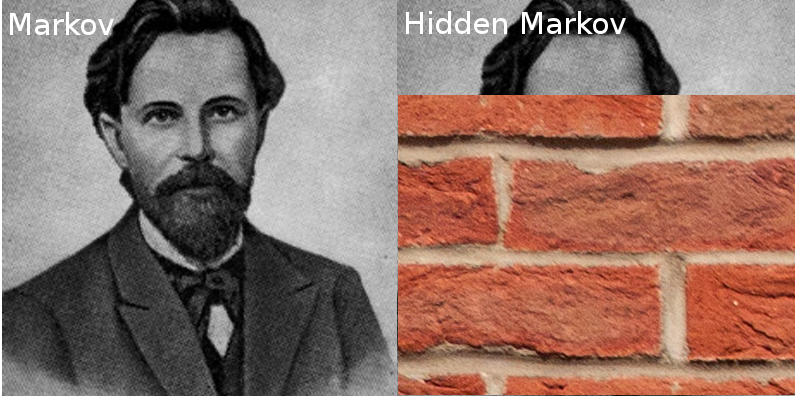
\includegraphics[width=10cm]{markov}
\end{frame}
\end{document}
